%\documentclass[notes,10pt,aspectratio=169]{beamer}
\documentclass[10pt,aspectratio=169]{beamer}

\usetheme[progressbar=frametitle]{metropolis}
\usecolortheme{rose}
\usecolortheme{default}

\usepackage[utf8]{inputenc}
\usepackage[T1]{fontenc}
\usepackage{lmodern}
\usepackage{xcolor}
\usepackage{tikz}
\usepackage{booktabs}
\usetikzlibrary{shapes.geometric, arrows, positioning}

\usepackage{adjustbox}
\setbeamertemplate{itemize item}[triangle]

\setbeamercolor{frametitle}{fg=black,bg=white}
\setbeamercolor{item}{fg= orange!80}
\setbeamercolor{button}{bg=orange, fg=white}

\usepackage[
  backend=biber,
  style=apa,
  citestyle=authoryear
]{biblatex}
\addbibresource{../references.bib}

\title{Meeting with Judy}

\author{%
 Lucas Condeza
\inst{1}
}
\institute{
  \inst{1} Yale University \\
}

\date{\today}

\begin{document}

%-------------------------------
\begin{frame}{Last meeting}
\begin{itemize}
    \item Last meeting:
    \begin{itemize}
    \item Presented research proposal on cross-selling in consumer credit markets
    \item Rationales for cross-selling: switching cost and information asymmetries 
    \item Judy suggested it could be interesting to look at the effect of \textbf{credit bureaus} on competition
\end{itemize}
\item Today's meeting:
\begin{itemize}
    \item A policy in Chile --- the \textbf{REDEC} (Registro de Deuda Consolidada) --- provides a natural experiment to study this
    \item Explain the policy and possible research questions
\end{itemize}
\end{itemize}
\end{frame}


%-------------------------------
\begin{frame}{The REDEC Policy}
\begin{itemize}
    \item \textbf{What:} Chile creates a centralized Consolidated Debt Registry (REDEC), managed by the financial regulator (CMF). Takes effect \textbf{April 1, 2026}.
    \item \textbf{Before REDEC:}
\begin{itemize}
    \item Banks shared positive credit info among themselves (N\'omina de Deudores)
    \item Non-bank lenders (retail stores, compensation funds, cooperatives) --- over \textbf{30\% of consumer credit} --- were excluded from this system
    \item Non-bank lenders had \textbf{no access} to bank credit histories
    \item Only negative info (delinquencies) shared publicly via Bolet\'in Comercial
\end{itemize}
    \item \textbf{After REDEC:}
\begin{itemize}
    \item \textbf{All} lenders (banks + non-banks) must report positive and negative credit info
    \item \textbf{All} registered lenders can access a borrower's full debt profile
\end{itemize}
\end{itemize}
\end{frame}

 \begin{frame}{Failure that policy aims to solve}
    \centering
    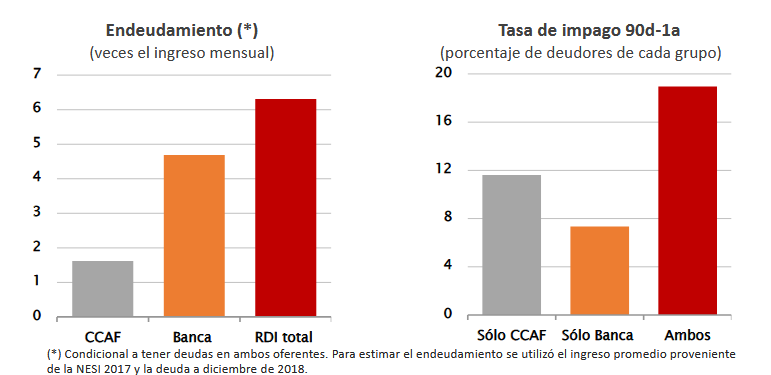
\includegraphics[width=0.65\textwidth]{../figures/Screenshots/BC 2019_2.png}
\begin{itemize}
    \item Hidden debt creates a screening problem: banks lend to applicants without knowing their total leverage at non-bank institutions. The gap in default rates between ``bank + non-bank'' and ``bank-only'' borrowers reflects the cost of this information asymmetry.
\end{itemize}
\end{frame}


%-------------------------------
\begin{frame}{Research Questions}
\begin{itemize}
    \item Main question: What are the effects of expanding credit information sharing on competition and welfare in consumer credit markets?
    \item Predictions:
    \begin{enumerate}
        \item Borrower mobility: Post-REDEC, ``good'' non-bank borrowers (no delinquencies) are more likely to obtain loans from banks, as their previously invisible repayment history becomes portable.
        \item Pricing: Good non-bank borrowers who switch to banks receive lower interest rates post-REDEC, as banks can now separate good from bad types instead of pooling.
        \item Loan quality: Default rates on new bank loans decrease post-REDEC, as banks screen out applicants with hidden non-bank delinquencies.
    \end{enumerate}
\end{itemize}
\end{frame}


%-------------------------------
\begin{frame}{Reduced-Form Regressions}
\begin{itemize}
    \item Credit access (sample: OCNB-only borrowers, $Good_i = \mathbf{1}[\text{no OCNB delinquencies}]$)
    $$NewBank_{it} = \beta^A \cdot (Post_t \times Good_i) + \gamma X_{it} + \delta_i + \theta_t + \varepsilon_{it}$$
    Expected: $\hat{\beta}^A > 0$ --- good types gain bank access once histories are visible

    \item Pricing 
    $$r_{ijt} = \beta^P \cdot (Post_t \times Good_i) + \gamma X_{it} + \mu_j + \theta_t + \varepsilon_{ijt}$$
    Expected: $\hat{\beta}^P < 0$ --- good types get lower rates (separating vs.\ pooling)

    \item Delinquency
    $$Delinq_{ijt} = \beta^D \cdot (Post_t \times OCNB\_Debt_i) + \gamma X_{it} + \mu_j + \theta_t + \varepsilon_{ijt}$$
    Expected: $\hat{\beta}^D < 0$ --- banks screen on OCNB debt, improving loan composition
\end{itemize}
\end{frame}




 
\end{document}
